\documentclass[11pt]{article}


\usepackage{fullpage}
\usepackage{graphicx}
\usepackage{amsmath}
\usepackage{amssymb}
\usepackage{amsthm}
\usepackage{fancyvrb}

\newcommand{\myname}{Mehshan Mustafa}

\newenvironment{theorem}[2][Theorem]{\begin{trivlist}
\item[\hskip \labelsep {\bfseries #1}\hskip \labelsep {\bfseries #2.}]}{\end{trivlist}}
\newenvironment{lemma}[2][Lemma]{\begin{trivlist}
\item[\hskip \labelsep {\bfseries #1}\hskip \labelsep {\bfseries #2.}]}{\end{trivlist}}
\newenvironment{exercise}[2][Exercise]{\begin{trivlist}
\item[\hskip \labelsep {\bfseries #1}\hskip \labelsep {\bfseries #2.}]}{\end{trivlist}}
\newenvironment{problem}[2][Problem]{\begin{trivlist}
\item[\hskip \labelsep {\bfseries #1}\hskip \labelsep {\bfseries #2.}]}{\end{trivlist}}
\newenvironment{question}[2][Question]{\begin{trivlist}
\item[\hskip \labelsep {\bfseries #1}\hskip \labelsep {\bfseries #2.}]}{\end{trivlist}}
\newenvironment{corollary}[2][Corollary]{\begin{trivlist}
\item[\hskip \labelsep {\bfseries #1}\hskip \labelsep {\bfseries #2.}]}{\end{trivlist}}
\newenvironment{solution}{\begin{proof}[Solution]}{\end{proof}}
\newenvironment{idea}[2][Proof Idea.]{\textit{#1} #2}



\parindent0in
\pagestyle{plain}
\thispagestyle{plain}

\newcommand{\dated}{\today}

\begin{document}

\textbf{Introduction to the Theory of
Computation}\hfill\textbf{\myname}\\[0.01in]
\textbf{Chapter 2: Context-Free Languages}\hfill\textbf{\dated}\\
\smallskip\hrule\bigskip

\begin{problem}{2.44}
If $A$ and $B$ are languages, define $A \lozenge B = \{xy \ | \ x \in A \ and \ y \in B \ and \ |x| = |y|\}$.
Show that if $A$ and $B$ are regular languages, then $A \lozenge B$ is a CFL.
\end{problem}

\begin{idea}
\begin{center}
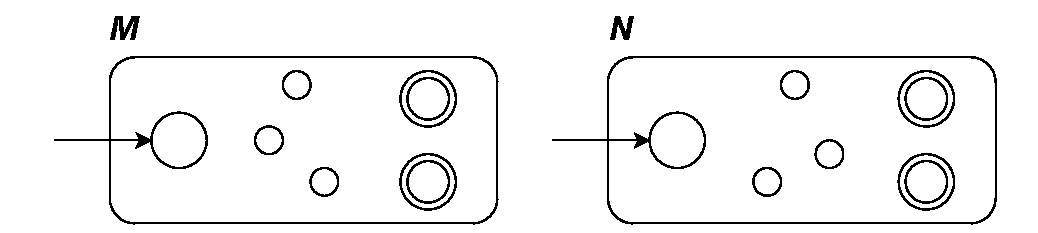
\includegraphics[scale=0.6]{Figures/Problem2.44a.pdf} \\
Let $M$ and $N$ be the DFAs that recognize the languages $A$ and $B$ respectively.
\end{center}
\begin{center}
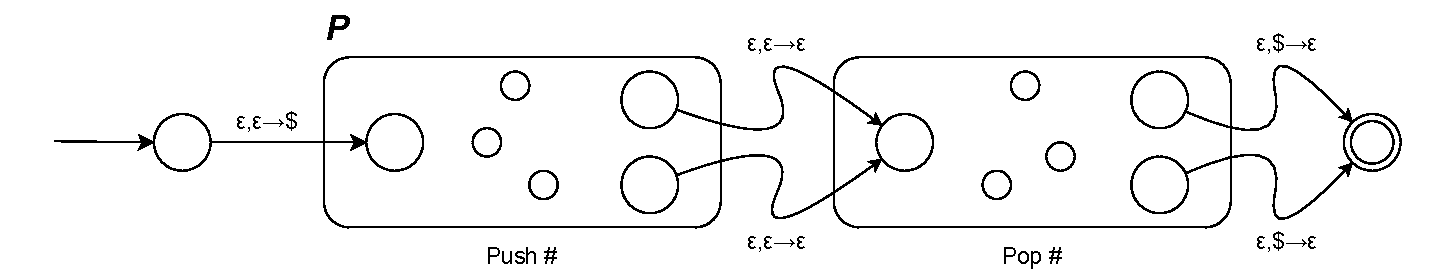
\includegraphics[scale=0.7]{Figures/Problem2.44b.pdf} \\
PDA $P$ that recognizes $A \lozenge B$.
\end{center}
\end{idea}

\begin{proof}
The proof is by construction. Let $M = (Q_m, \Sigma_m, \delta_m, q_m, F_m)$ be the DFA that recognizes $A$, and $N = (Q_n, \Sigma_n, \delta_n, q_n, F_n)$ be the DFA that recognizes $B$. Construct the PDA $P = (Q, \Sigma, \Gamma, \delta, q_0, F)$ as follows:
\begin{enumerate}
\item $Q = Q_m \cup Q_n \cup \{q_s, q_a\}$. The state $q_s$ is the new start state, and $q_a$ is the new accept state.
\item $\Sigma = \Sigma_m \cup \Sigma_n$
\item $\Gamma = \{\#, \textdollar\}$
\item $q_0 = q_s$
\item $F = \{q_a\}$
\item Define $\delta(q, a, s)$ so that for any $q \in Q$, any $a \in \Sigma_{\epsilon}$, and any $s \in \Gamma_{\epsilon}$:
\end{enumerate}
\begin{center}
$\displaystyle \delta(q, a, s) \ =\begin{cases}
\{ (q_m, \textdollar) \} & q = q_s, \ a = \epsilon \ and \ s = \epsilon  \\
\{ (\delta_m(q, a), \#) \} & q \in Q_m, \ a \in \Sigma_m, \ and \ s = \epsilon \\
\{ (q_n, \epsilon) \} & q \in F_m, \ a = \epsilon, \ and \ s = \epsilon \\
\{ (\delta_n(q, a), \epsilon) \} & q \in Q_n, \ a \in \Sigma_n, \ and \ s = \# \\
\{ (q_s, \epsilon) \} & q \in F_n, \ a = \epsilon, \ and \ s = \textdollar
\end{cases} \ \ $
\end{center}
\end{proof}

\end{document}
